\documentclass[a4paper]{article}
\usepackage{geometry}
\geometry{margin=1in}

\usepackage[english]{babel}
\usepackage[utf8]{inputenc}
\usepackage{amsmath}
\usepackage{graphicx}
\usepackage[colorinlistoftodos]{todonotes}
\usepackage{gensymb}
\usepackage{hyperref}
\usepackage[T1]{fontenc}
\usepackage{lmodern}
\usepackage{minted}
\usepackage{url}
\usepackage{fancyhdr}
\usepackage{wrapfig}

\setlength{\parskip}{0.7em}
\title{ \textbf{Introduction to Programming \& The Internet of Things} \\
Module 4: Data Acquisition \& The Internet of Things \vspace{-5ex} \\
}
\date{}

\begin{document}
\maketitle
\thispagestyle{fancy}
\lhead{University of Texas at Austin \\ Civil, Architectural, and Environmental Engineering \\ Material curated by Thomas Dougherty}
\rhead{Professor Dr. Zoltan Nagy \\ https://nagy.caee.utexas.edu \\ Fall 2018}

\section{Modules Background}
There is a pervasive need to study the performance of built structures and their abilities to provide occupants with comfort in an efficient manner. The Internet of Things (IoT) provides methods of obtaining and studying data about our built environments. As such, these modules introduce civil, architectural, and environmental engineers to tropics of electrical engineering. Students will gather the abilities needed to program and deploy necessary sensors in the Internet of Things (IoT), as well as gain the ability to gather and analyze data collected.

\tableofcontents
\newpage

\section{Introduction}
\label{sec:introduction}

In this module, we're going to explore ways to collect data and analyze it. From a high level, we're going to talk about where you should look when starting to use a sensor, how to incorporate libraries into your Arduino code, and how to format this data in a way we can use with something like excel. Likewise, we'll touch on a few different protocols and Often you'll find that there are already a lot of great utilities to use that will expedite the process of connecting sensors and make our lives a lot easier. Without further ado, let's get coding!

\section{Protocols}
\subsubsection{Analog Voltage / Variable Resistance}

\label{fig:a_vol}
\begin{wrapfigure}{r}{0.3\textwidth}
  \begin{center}
    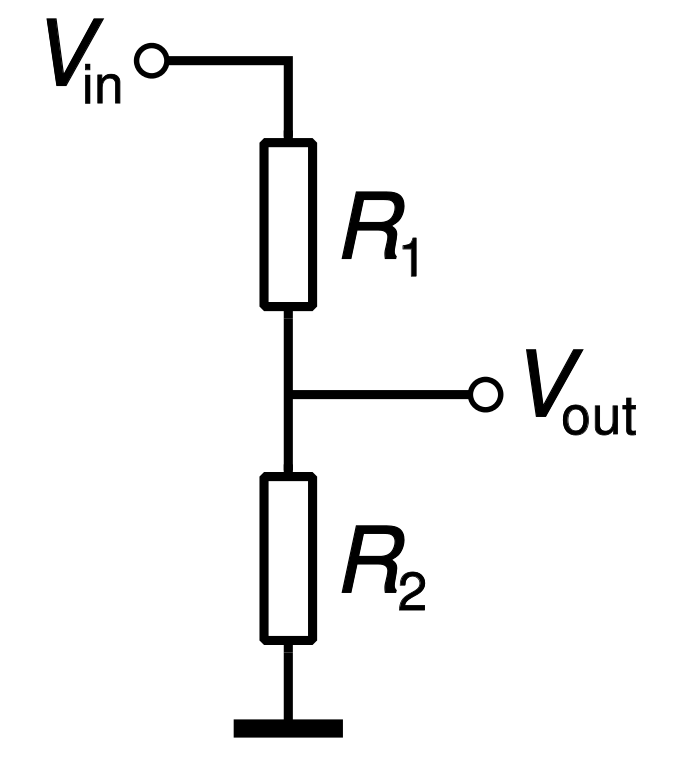
\includegraphics[width=0.3\textwidth]{voltage_divider.png}
  \end{center}
  \caption{Analog Voltage Example Setup}
\end{wrapfigure}

The easiest and most basic form of collecting data is analog voltage. Many sensors like photo resistors (light sensitivity) or hall effect sensors (magnetic field) usually output analog voltage. This means that the sensor has been able to convert some physical system like pressure or light into a change in resistance. Putting this into a voltage divider, where it's visible that as one of the R values changes the Vout changes proportionally).  The Arduino comes with a few analog voltage reading inputs, which makes reading analog voltages extremely easy.

\newline
\noindent
\textbf{Pros:} Extremely easy, super rapid prototyping.
\newline \noindent
\textbf{Cons:} Not totally supported, requires more pins, perhaps voltage regulation.

\subsubsection{I2C}

\label{fig:spi}
\begin{wrapfigure}{l}{0.7\textwidth}
  \begin{center}
    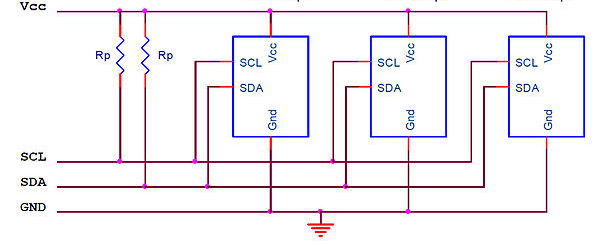
\includegraphics[width=0.7\textwidth]{I2C_bus.jpg}
  \end{center}
  \caption{Example of I2C Configuration}
\end{wrapfigure}

There are a few protocols with are a lot more popular in industry than others, and the crowd favorite for ease of use and functionality is $I^2C$ (Eye - Squared - C). This is also called "Two wire interface", and one of the benefits of this protocol is that it can be daisy chained to contain a number of devices using just two main wires for transmission.

This configuration uses "pull-up" resistors, which basically tells us that our transmission voltage will be high unless it is pulled low by the slave devices. In English? Think about how a city bus works. There are a bunch of people who need to communicate to the bus driver when they need to get off. To do so, they reach up and give a tug on the cable. This tug communicates to the bus driver some kind of information. After the person tugs the cable, it is restored to the original position of being relatively taught near the top of the bus ceiling. It might seem like this explanation is a bit drawn out, but there are a lot of parallels in $I^2C$ communication.

When you connect a peripheral device (any kind of sensor or communication system) to the main device (what is called the "master" node), it's like the sensor is getting on the bus (which is conveniently also called the "bus" line). When it needs to communicate to the master node, it also pulls the line down. But instead of pulling the cable low, it's pulling the voltage line low. To restore the voltage to the original "high" voltage, a "pull-up" resistor is used. This allows the line to be restored to the original high voltage when our peripheral isn't asserting it low. Sometimes the device has these pull-up resistors built into a circuit board (as is our case for the tsl2561) so we don't need to think about this too much.

If you'd like to do more research on how $I^2C$ works, here's a good place to start \cite{i2c}. Luckily, most of the necessary code for communicating with sensors using $I^2C$ is already written, you just need to know where to find it!

\newline \noindent
\textbf{Pros:} Easy, generally universally supported with sensors, only two wires for interfacing,
\newline \noindent
\textbf{Cons:} Small learning curve, requires compatible sensors (although they generally are), and consistent voltage source, sometimes requires pull-up resistor.

\subsubsection{SPI}
\label{sec:protocol}
\begin{wrapfigure}{r}{0.4\textwidth}
  \begin{center}
    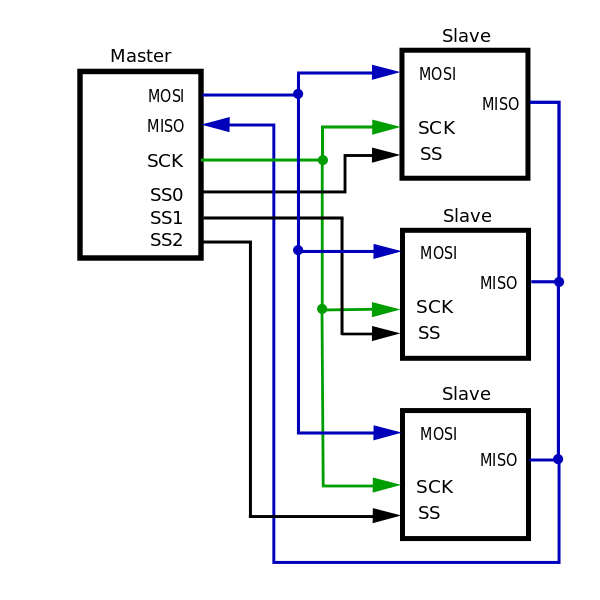
\includegraphics[width=0.4\textwidth]{spi.png}
  \end{center}
  \caption{Example of SPI Configuration}
\end{wrapfigure}

SPI (S - P - Eye) is good when you need a high data transmission. Think something like a camera, screen, or lidar sensor. The way it can achieve this high data transfer, however, is through an increased number of wires.

\newline \noindent
\textbf{Pros:} Great for high data transmission systems, generally supported.
\newline \noindent
\textbf{Cons:} Requires more pins, higher learning curve, not as commonly supported, \textbf{requires microcontroller that's compatible}.

\subsection{Example}
\subsubsection{Problem and Research}
Let's say you want to hook up a light sensor. The \href{https://www.adafruit.com/product/439}{tsl2561} for example! Where you you start? Often, the first place you'll look is on github. By searching "tsl2561" in Google, a github repository is usually the first thing that pops up. "Github" is a great resource that will come up a lot when coding, so it's good to have a basic idea of what it does. Github is a place for sharing and working collaboratively on code, and is used widely in both industry and in academia. It's quite famous for its version control system, which saves every iteration of the code over time (so if you mess up, there's an old copy). In this case, we're capitalizing on the availability of public code that github provides.

I found this github library using google:
\cite{TSL2561_Github}, which we're going to use in our system as a primary reference and tool. Likewise, you can reference this spec sheet if you'd like to find information about limitations and operating principles for this sensor: \cite{TSL2561_Specs}.

\section{Simulating Tools}
Once you have all of the necessary resources gathered, it's time to start building our system. Often it's useful to simulate a circuit before building it. A great tool is provided by Autodesk \cite{circuit_tool}. At the time of writing, there is a reasonably sized library of prebuilt sensor code from which you can find inspiration. Likewise, there's a program called Fritzing \cite{fritzing} which offers much of the same simulation setup and perhaps even more supported devices.

\section{Arduino IDE}
The Arduino platform was chosen for these modules in large part because of their accessibility, ease of use, and free software.

The Arduino software \cite{arduino} contains all of the software you'll need, with support for every platform. It is \textbf{highly} recommended that you download the software if you would like to work within the Ardunio platform. After we've downloaded the software, it should look something like figure \ref{fig:a_ide}! 

\begin{figure}
\centering
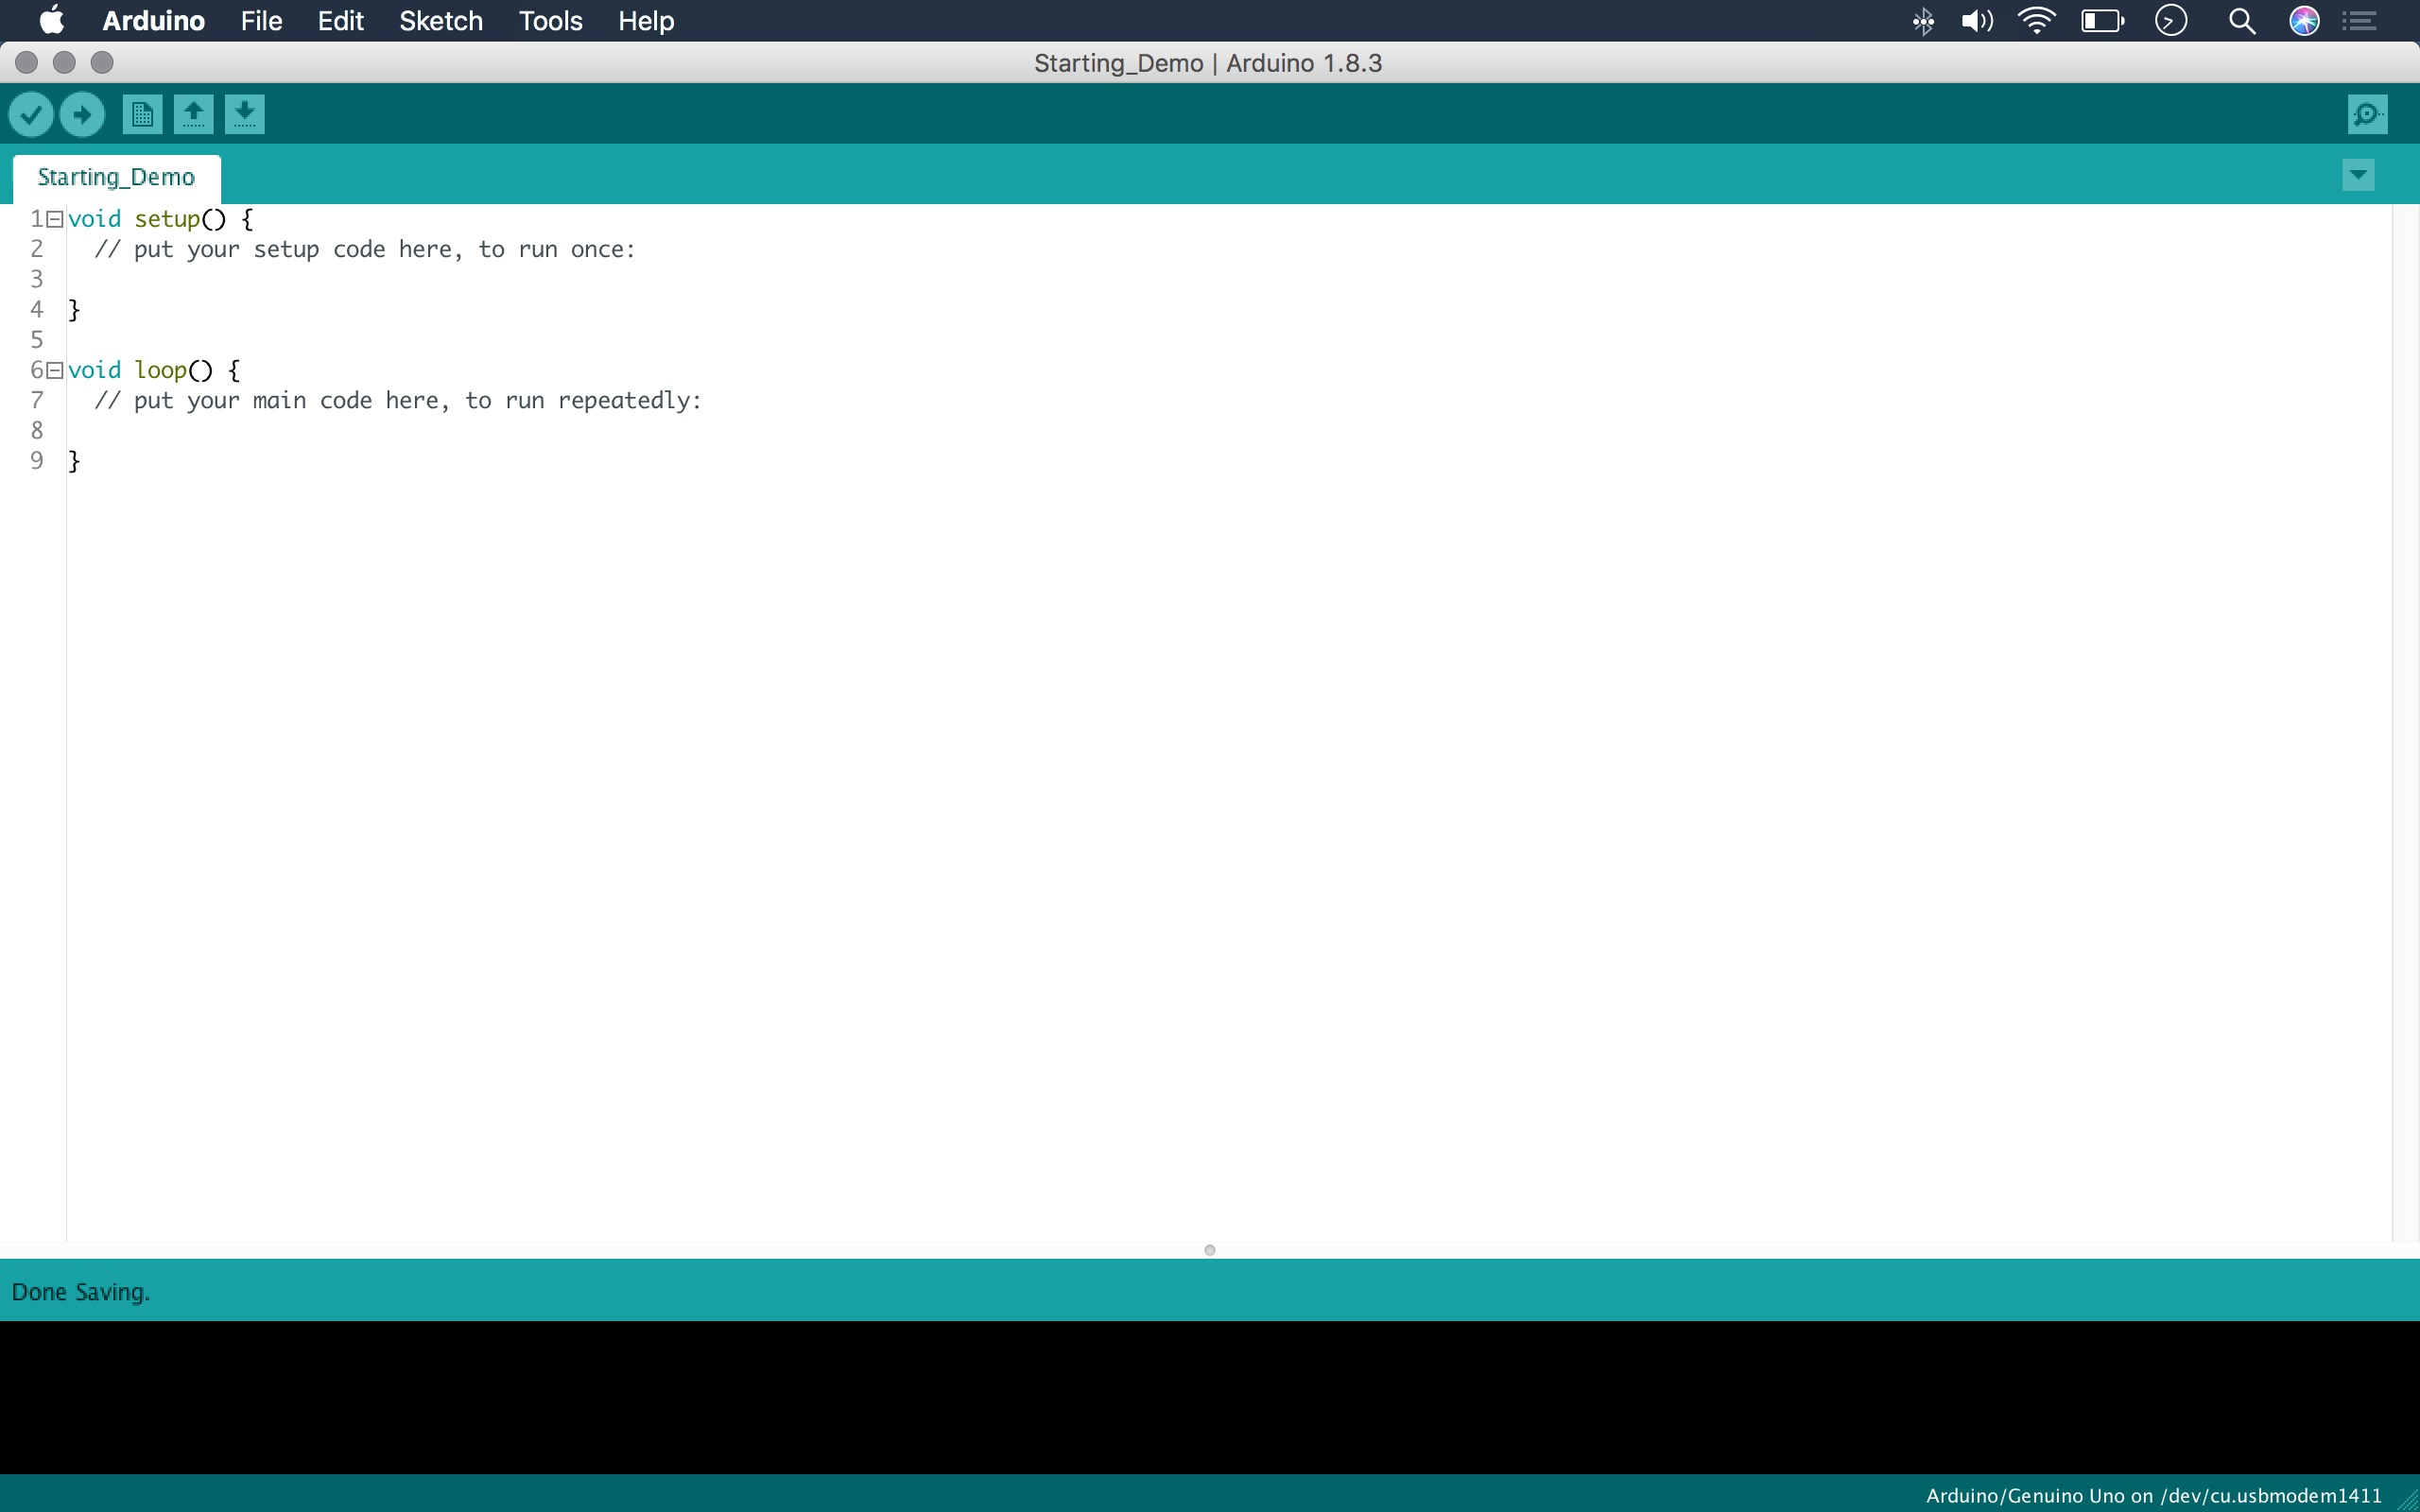
\includegraphics[width=1\textwidth]{a_ide.jpg}
\caption{Blank Arduino IDE.}
\label{fig:a_ide}
\end{figure}

\subsubsection{Libraries using the Arduino IDE}
Some of the more popular and common libraries have local support for them from within the Arduino IDE. The hookup guide on Adafruit's website actually shows this process quite clearly: \cite{arduino_guide}. \textbf{This is the easiest way} to get a sensor up and running if available. If it's not a highly supported sensor like those on Adafruit, the next place to look is if the sensor has code up and running on Github.

\subsubsection{From Github to the Ardunio}
Downloading a zip file of the repository from Github will give you a folder full of files. See figure \ref{fig:download_help} for where to do this on github's website. Once you download your file, it will be found in your "Downloads" folder as "Adafruit\_TSL2561-master.zip". Here are the steps we need to take in order to have our Ardunio IDE see this and allow us to run this code on the Ardunio:

\begin{enumerate}
  \item Double clicking this on a mac will "unzip" the file, and the same can be done with Windows by right clicking and selecting "Extract All".
  \item You'll now find that there's a file called "Adafruit\_TSL2561-master" in the same location on your computer which is a folder (or "directory"). Let's rename this to remove the "-master", so our final folder name is "Adafruit\_TSL2561".
  \item The final step is to move this folder into the place our Arduino app will be expecting to see it. On a mac, this location can be found in your "Documents" folder. Opening your finder, you'll find this on the left sidebar. See figure \ref{fig:docs_location} for a guide. On a PC, this libraries folder will be located in "Documents/My Documents". In either case, if the folder doesn't exist then make it in this location.
  \item Drag this folder (Adafruit\_TSL2561) into the Arduino/libraries folder. Now you'll be able to find the script in your Ardunio IDE!
\end{enumerate}

\noindent
If these steps didn't work for you, then I'd recommend consulting this guide \cite{arduino_library_guide}. In general, Adafruit is going to be a great resource for troubleshooting and step by step guides for your sensors.

\begin{figure}
\centering
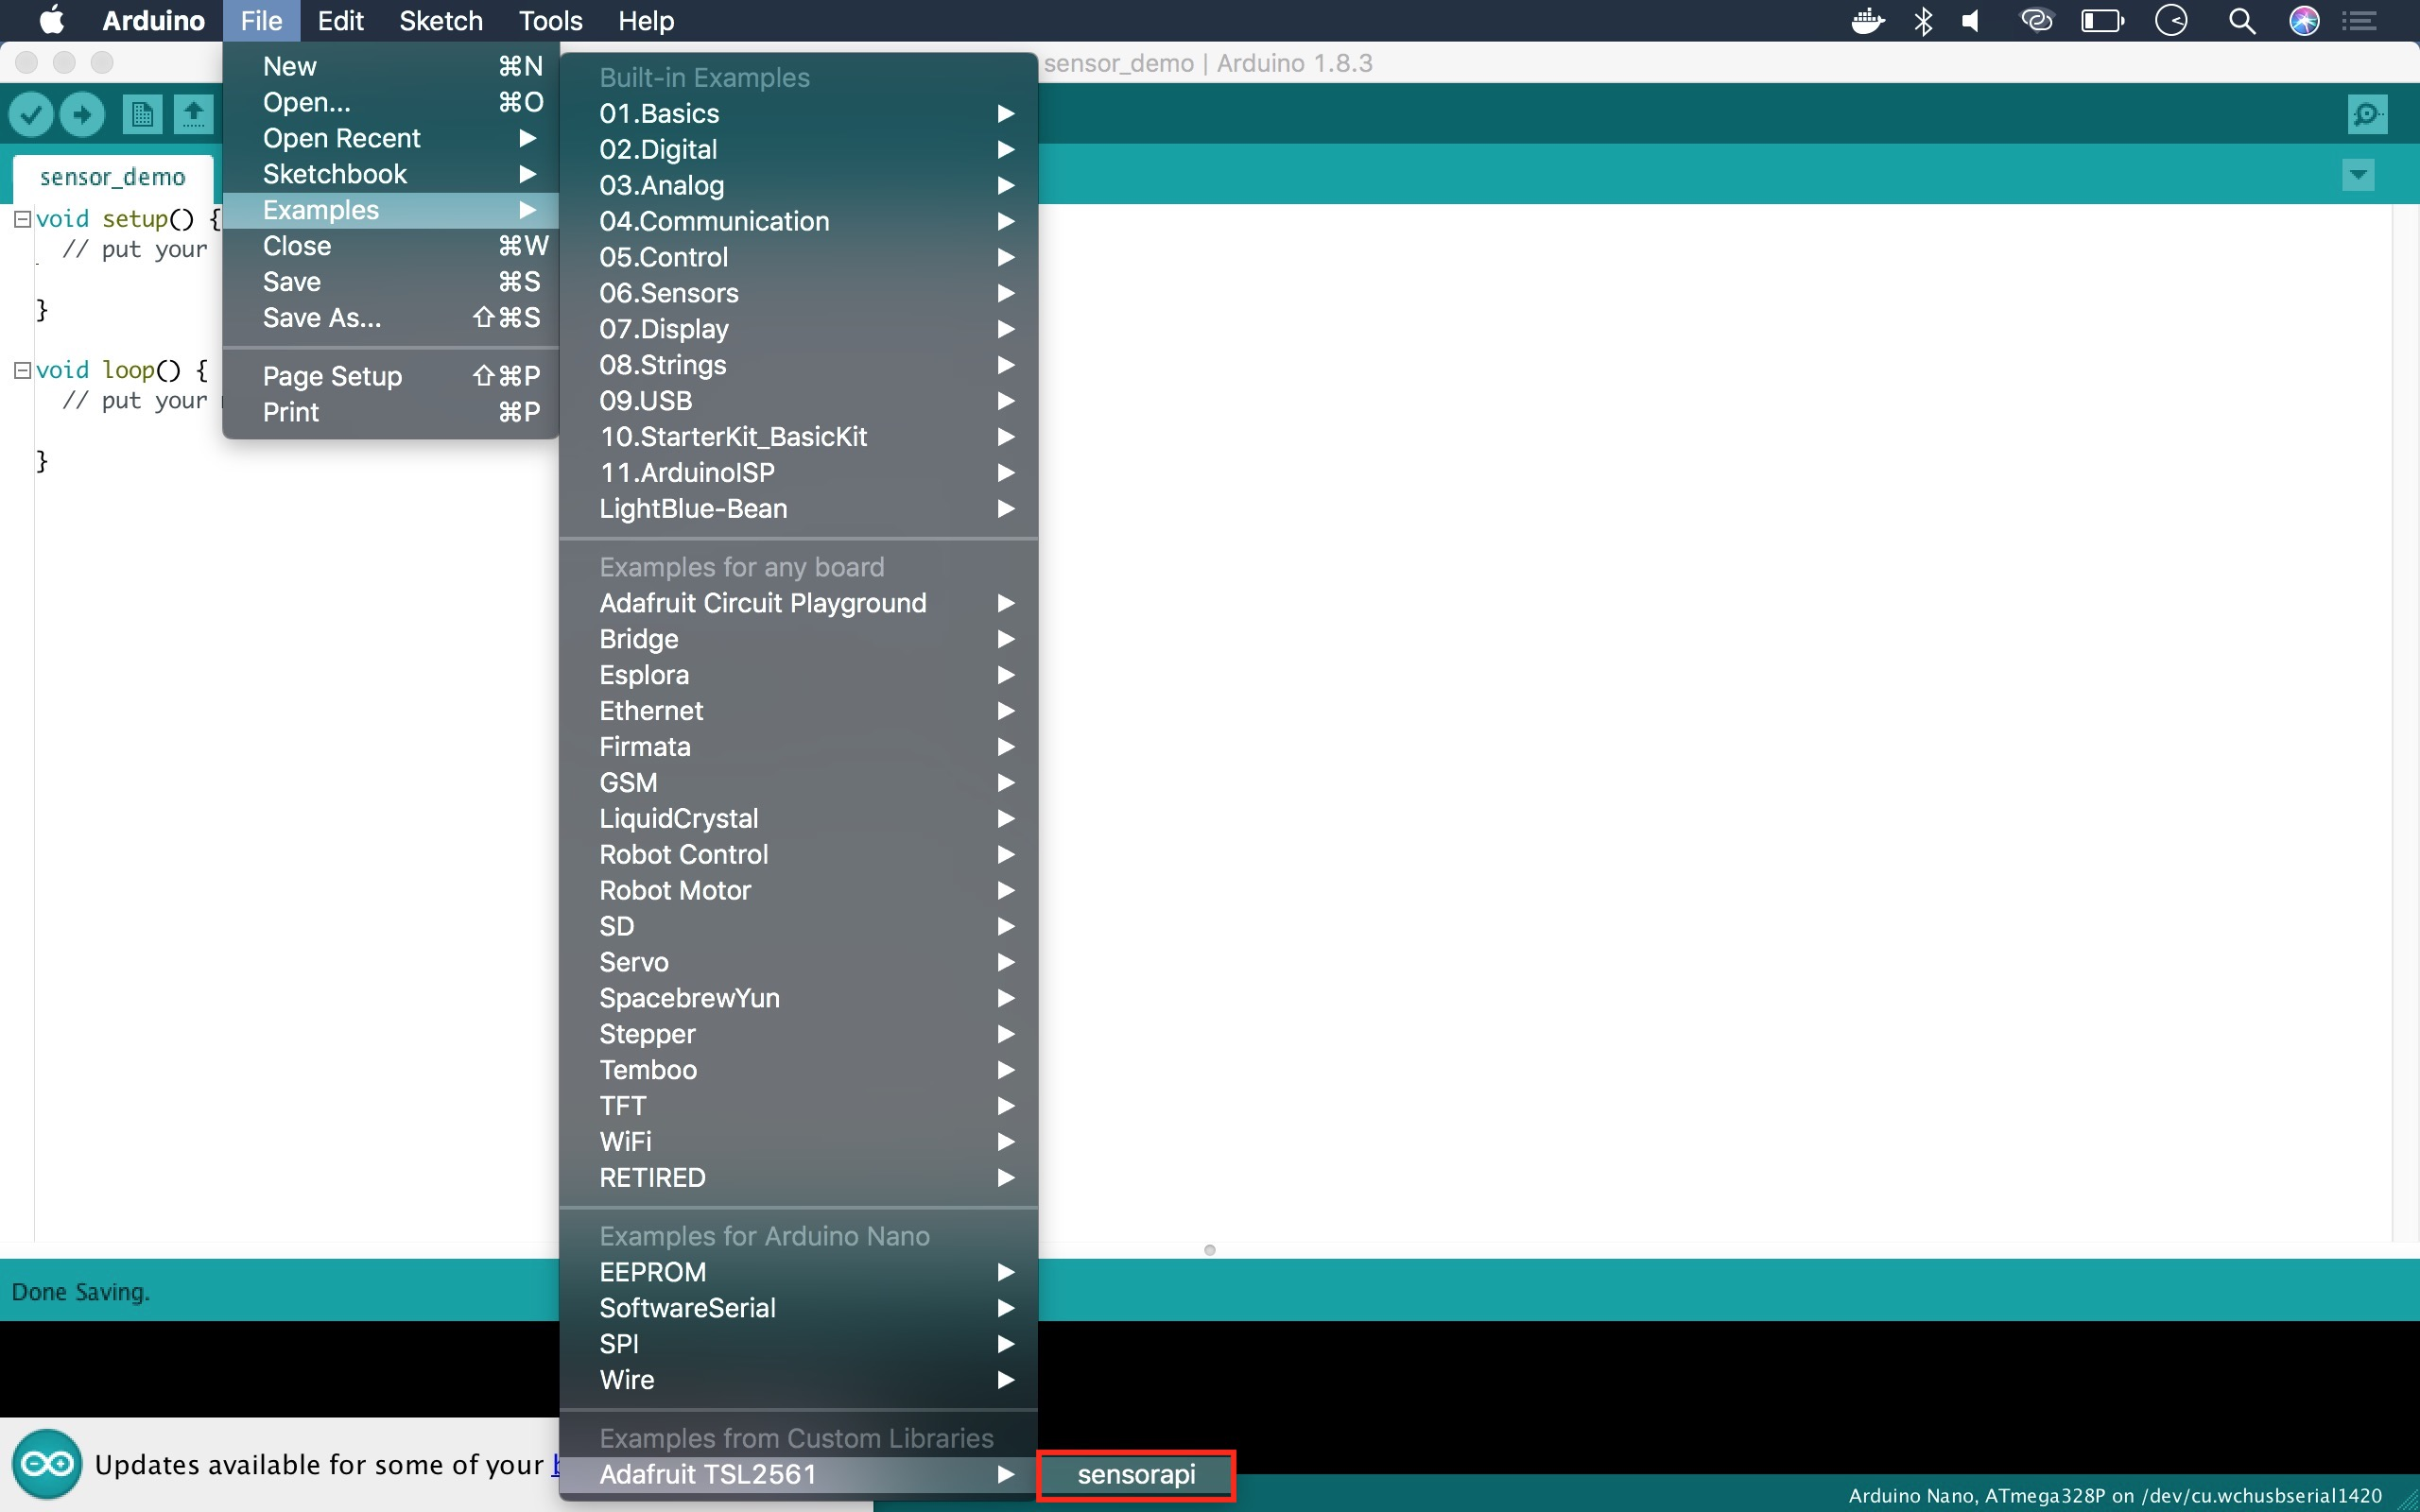
\includegraphics[width=1\textwidth]{file_location.jpg}
\caption{\label{fig:file_location}TSL2561 example file location.}
\end{figure}

\begin{figure}
\centering
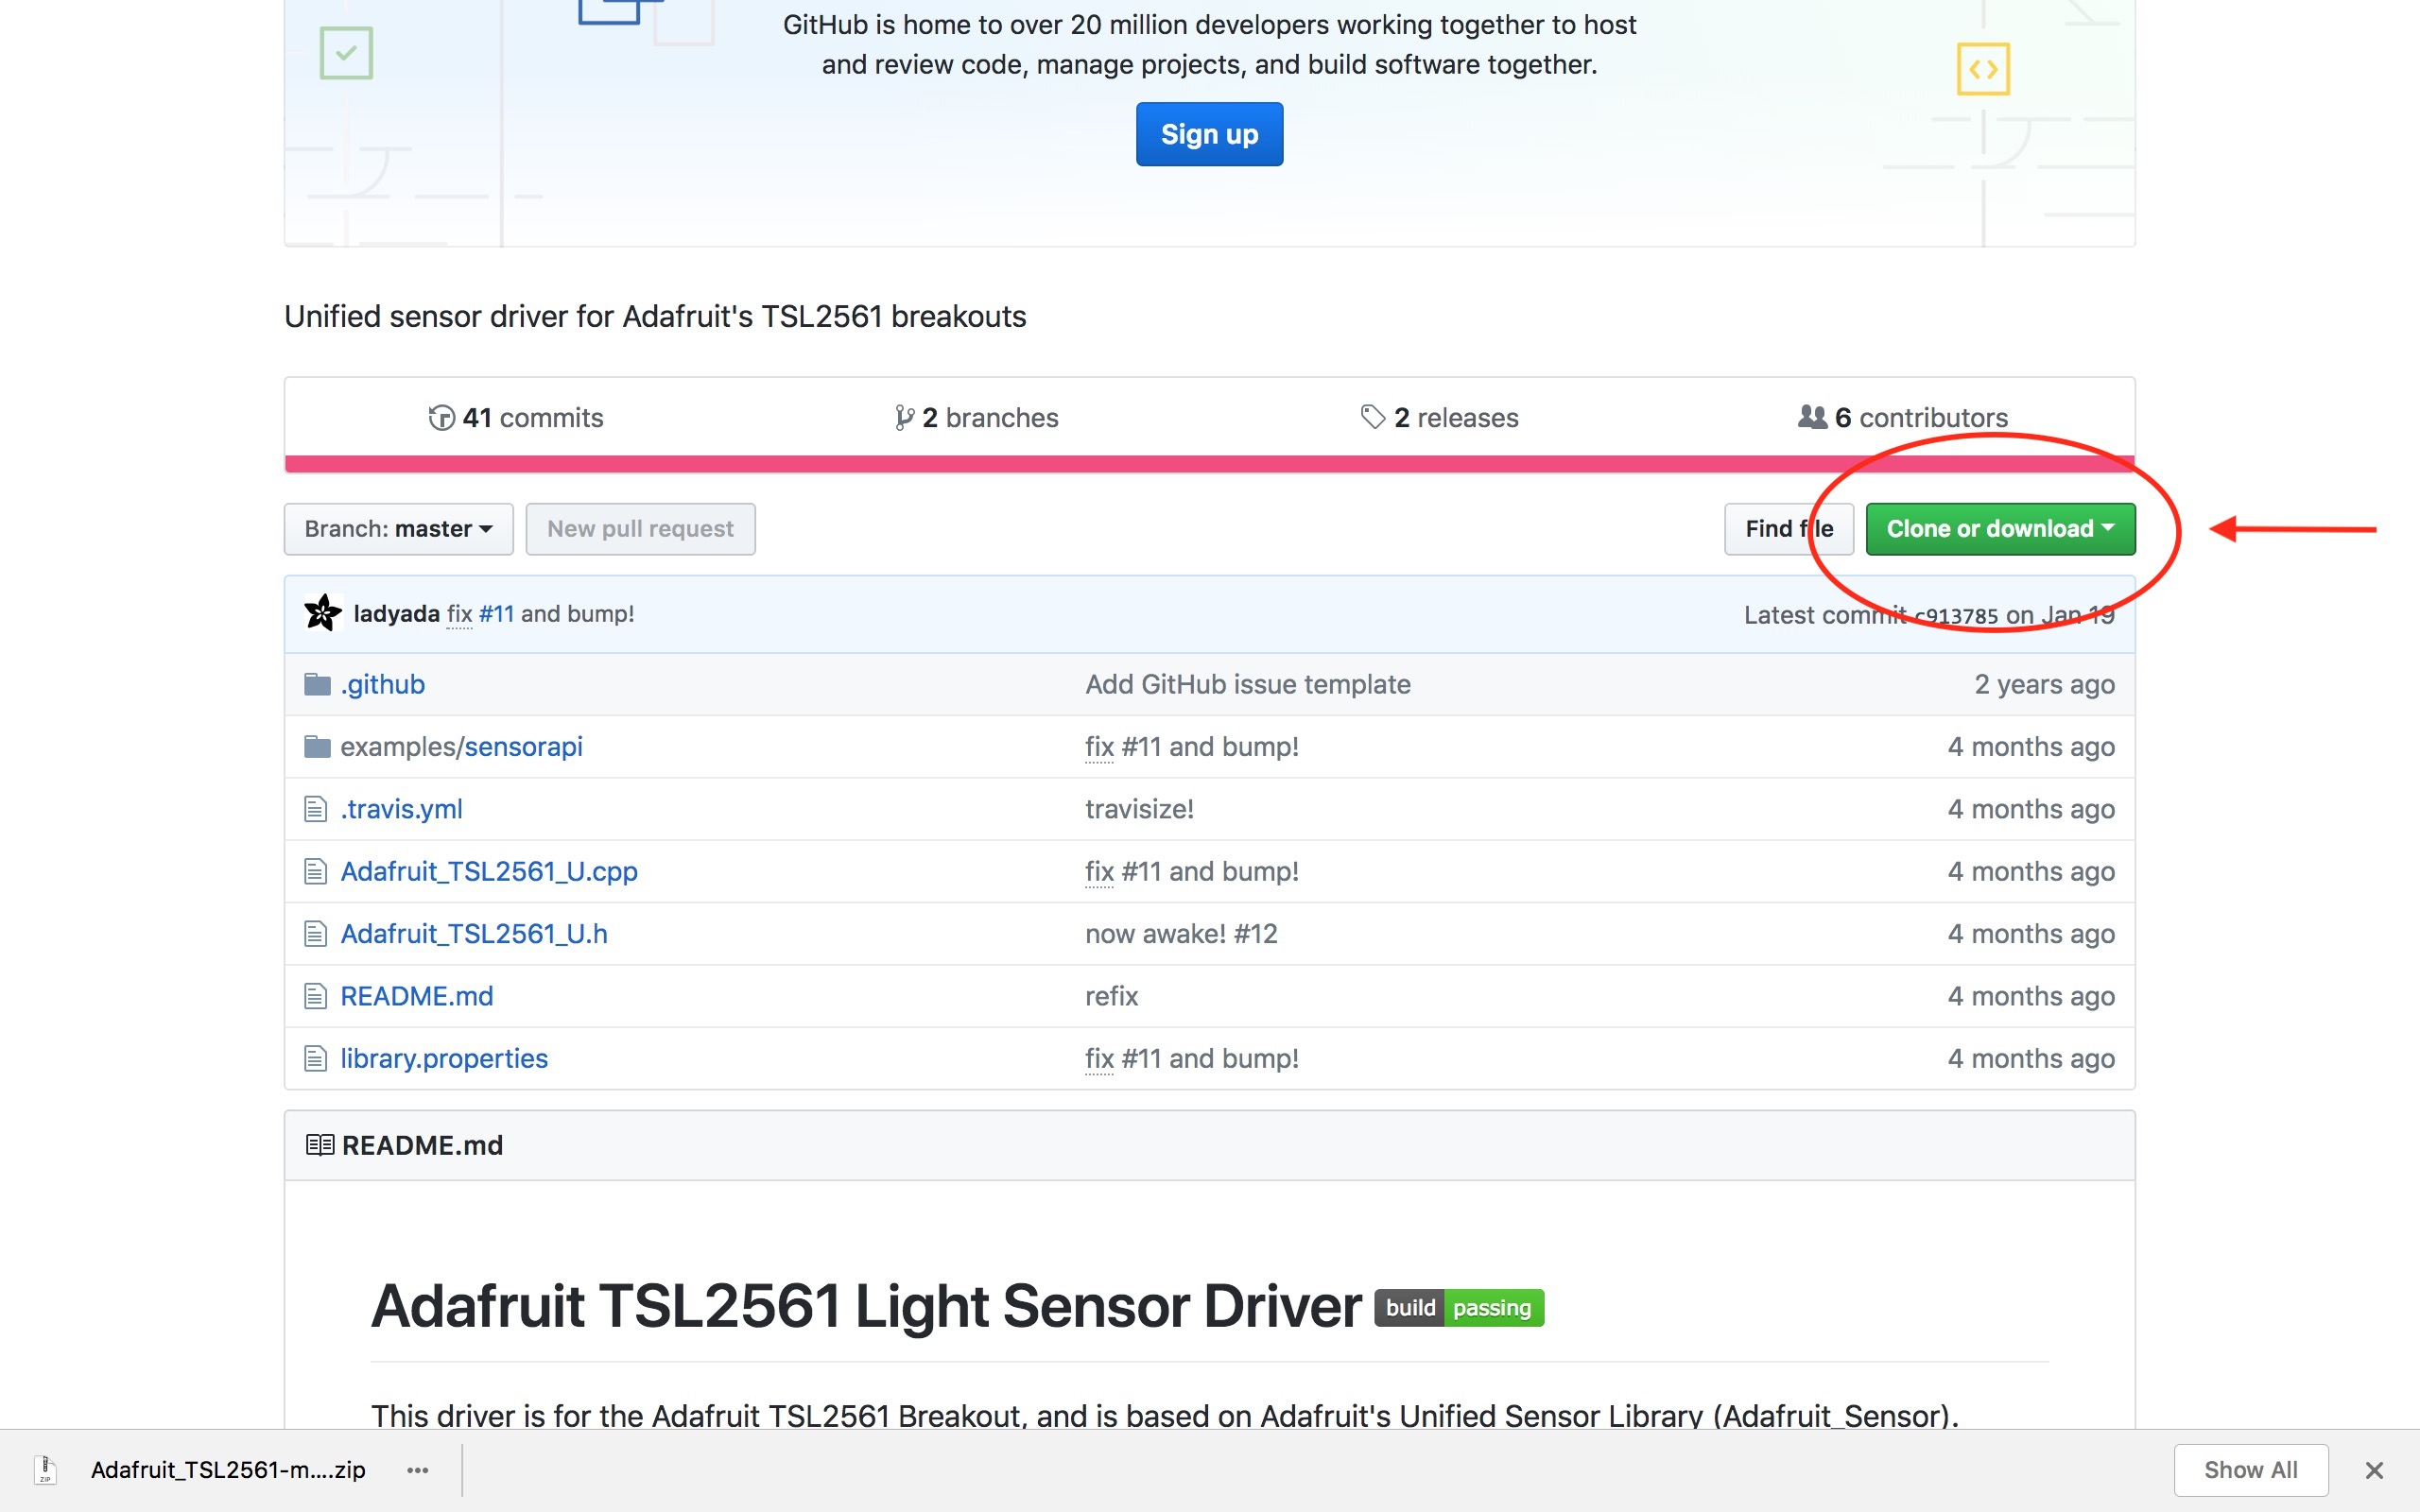
\includegraphics[width=1\textwidth]{Download_TSL2561.jpg}
\caption{\label{fig:download_help}Download Here.}
\end{figure}

\begin{figure}
\centering
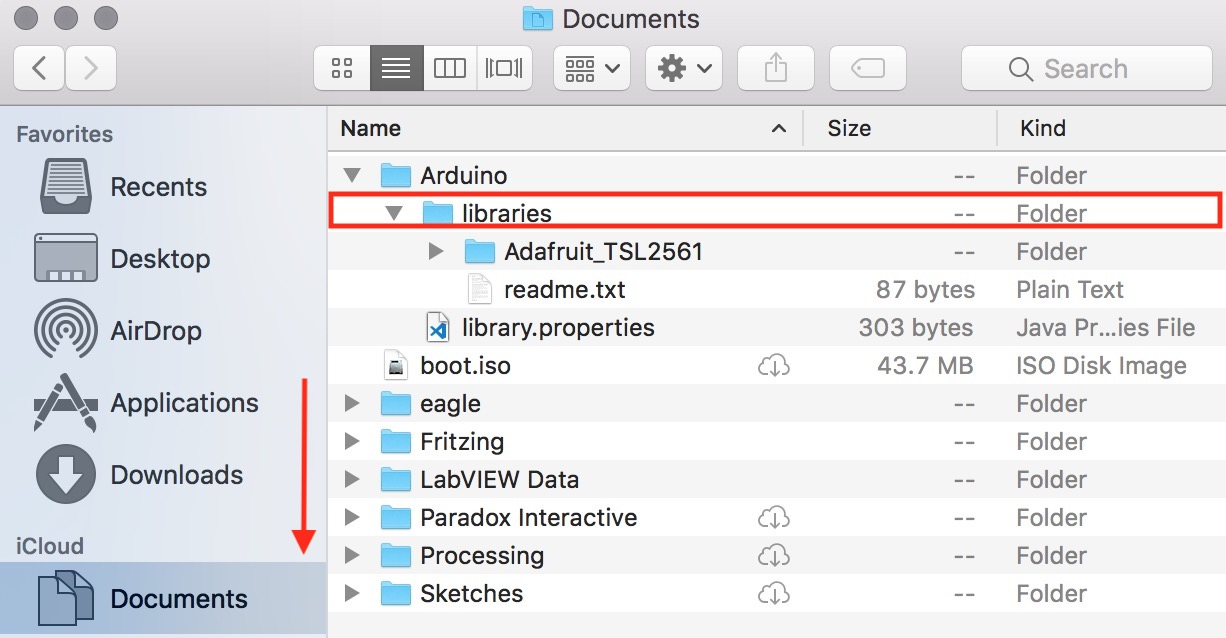
\includegraphics[width=1\textwidth]{Documents_location.jpg}
\caption{\label{fig:docs_location}Ardunio Folder Location - Mac.}
\end{figure}

\begin{figure}
\centering
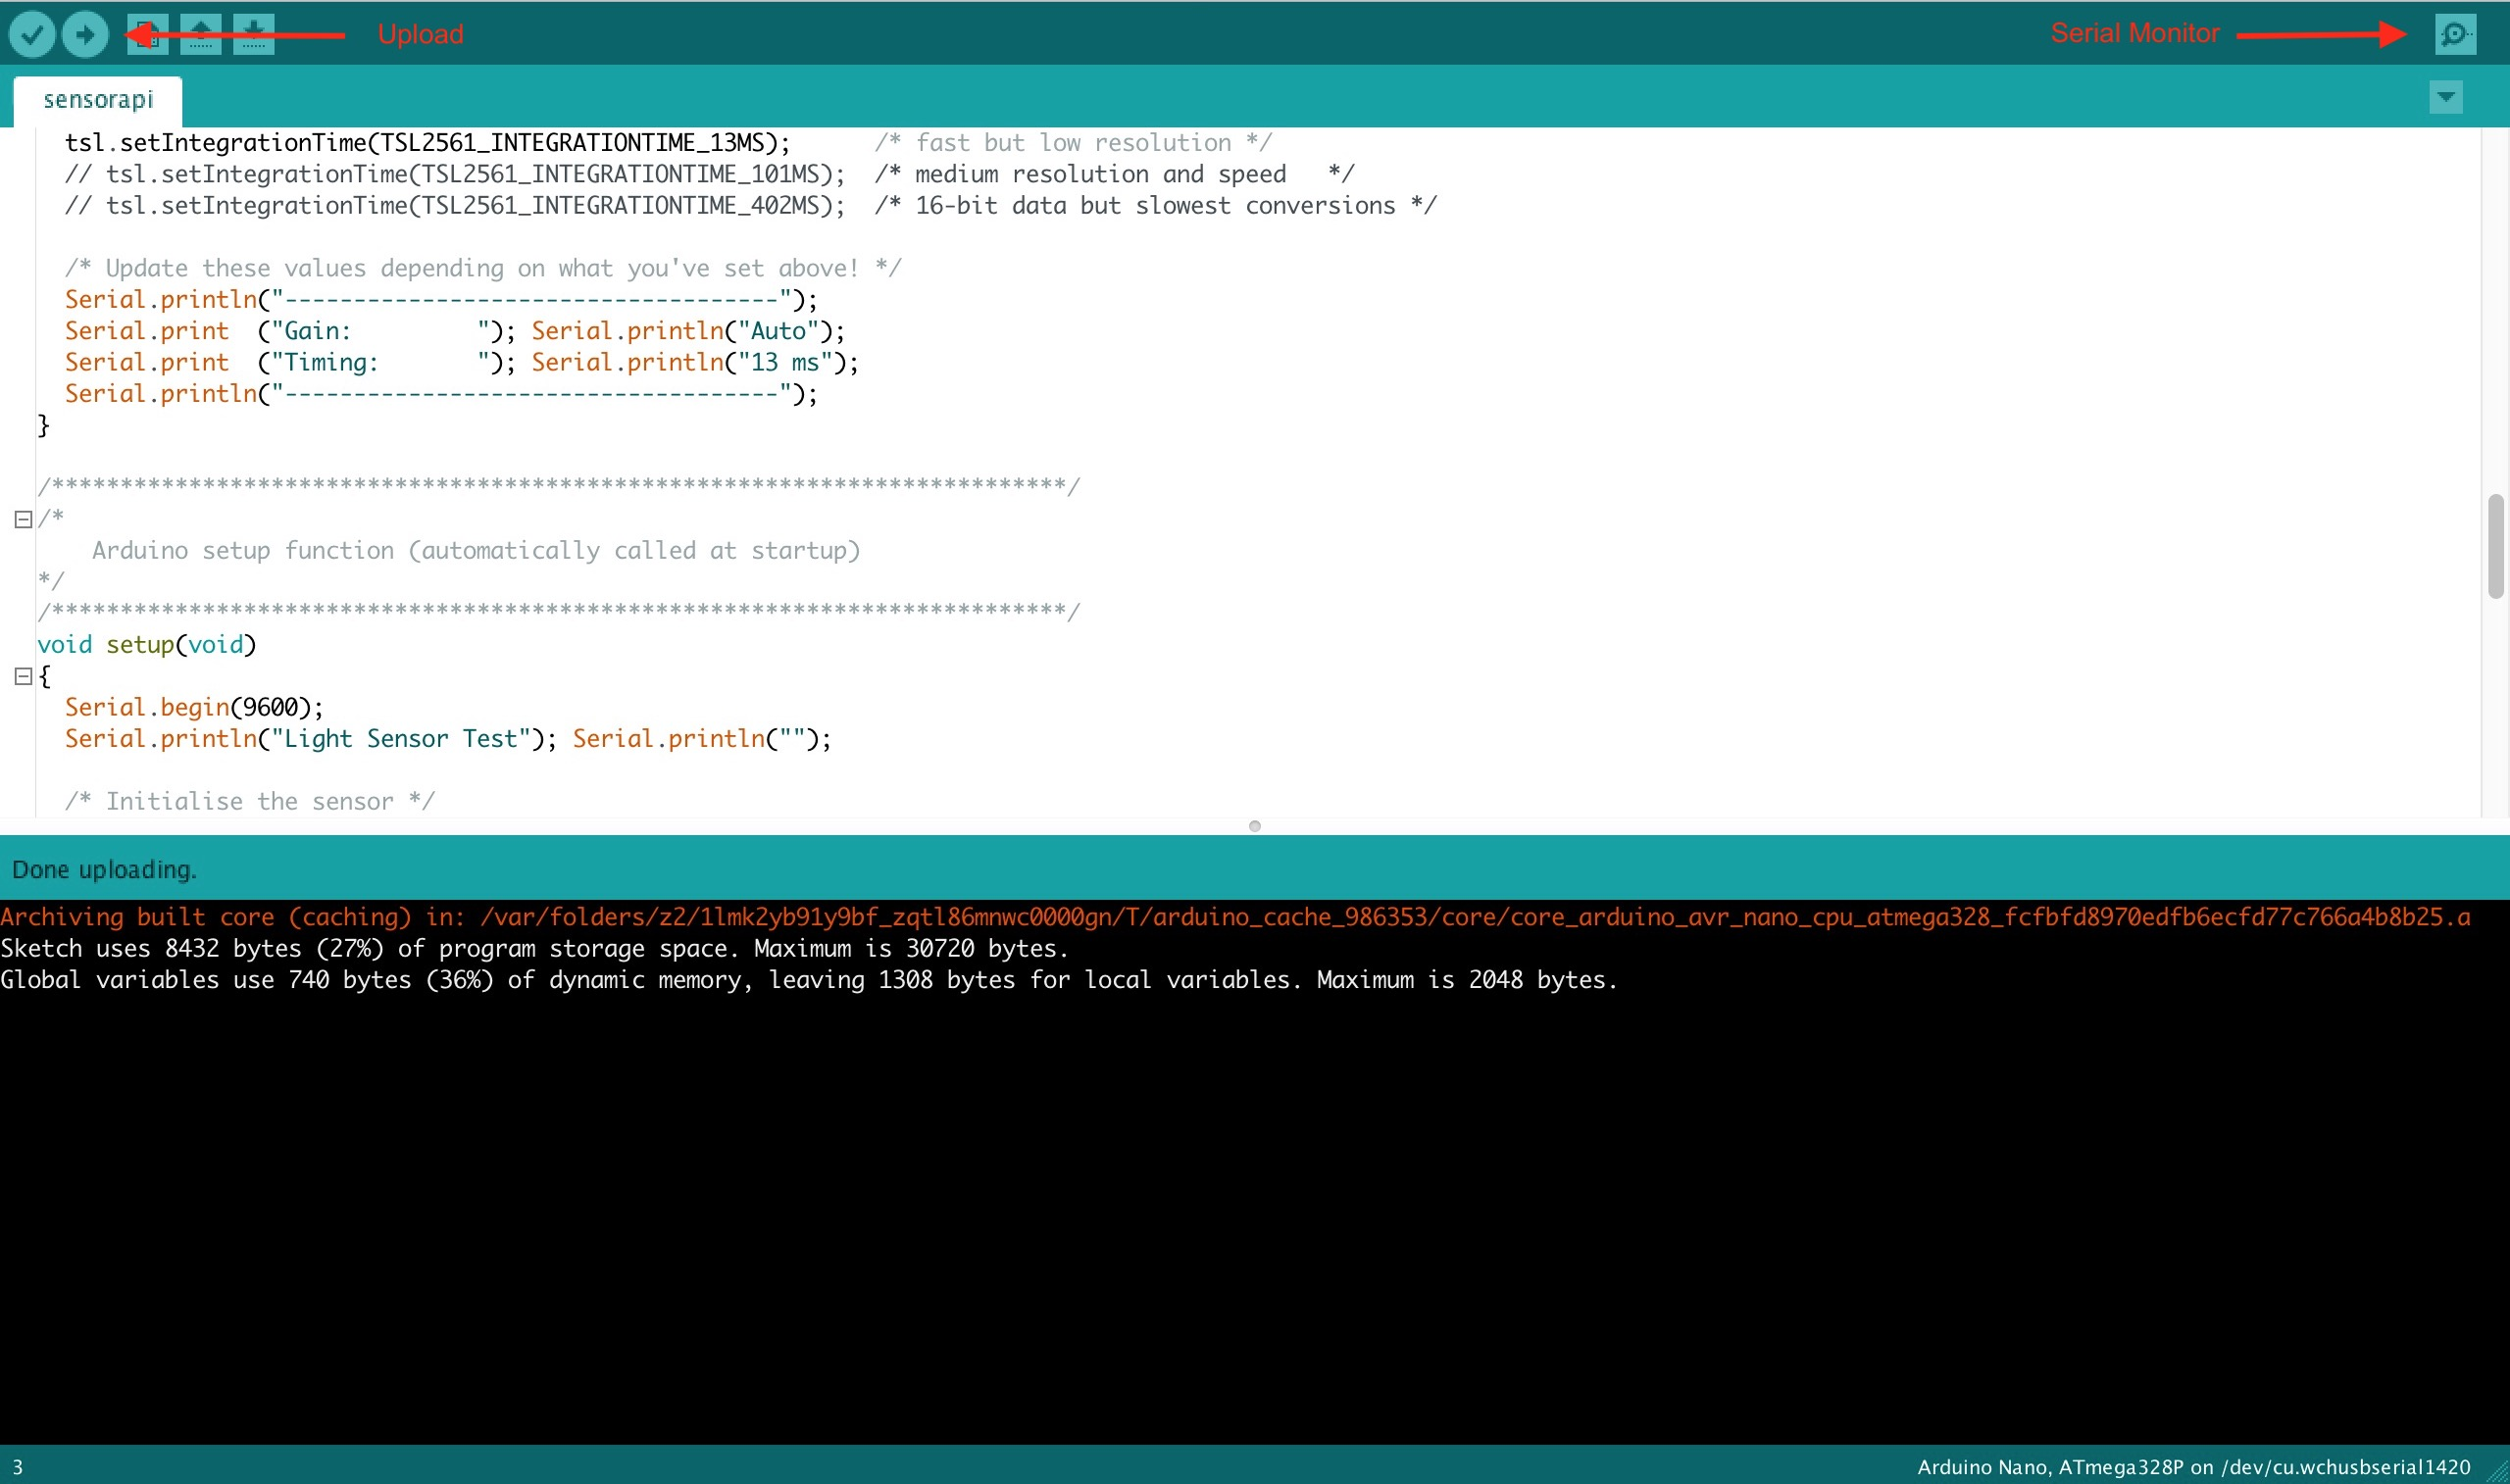
\includegraphics[width=1\textwidth]{run_serial.jpg}
\caption{\label{fig:run_serial}Location of run button and serial monitor.}
\end{figure}

\section{Running and Monitoring Data}
The example code given in sensorapi is feeding values to the serial monitor (See figure \ref{fig:run_serial}), which basically means it's sending every value it gets to your computer through the cable. We can see this by clicking on the "Serial Monitor" button in the top right of the Arduino IDE (it looks like a magnifying glass). Run the code and then look at the serial monitor to verify that your sensor is up and running and the values seem appropriate. You'll know the code has run correctly when you see the two lines 
Sketch uses... and Global variables... that you see in figure \ref{fig:run_serial}.

\subsection{Common Errors}
The Arduino IDE needs to make sure it's looking for your physical Arduino computer in the right place. After you plug an Arduino Uno into your computer via USB, your computer will recognize that there's something in the USB socket. Likewise, it needs to know which kind of computer you're plugging in so it can upload the right way. Both of these issues are explained in this walk through \cite{arduino_error_walkthrough}.

\section{Recording Data}
\textbf{The easiest and quickest way to record data is by copying what's in the serial monitor and pasting it into excel.} This is probably the way you'll want to go if you're testing a sensor for a system. If you're recording long-term data, this might be less ideal. For those cases, you'll more than likely want to use SD card storage. This offers more permanent and larger data capturing ability.

Given what you've learned already with I2c, Github, and the Arduino IDE, I think it's safe to say you're ready to build a data logger! This guide might come in handy for that project \cite{arduino_datalogger}. Likewise, there are some prebuilt arduino boards with SD card support \cite{arduino_sd}, which could be a good option when long term storage is necessary. Remember that you're probably not the first person to run into any technical issues so look online if you get stuck!

\section{Example Questions}
\subsection{Light}
Use a photo-resistor \cite{photoresistor}, build a system capable of measuring light intensity. \cite{photoresistor_guide}

\subsection{Air Quality}
While Volatile Organic Compounds (VOCs) \cite{voc} aren't exactly the perfect metric for measuring air quality, they're primary components in smells, plant communication, and might give some indication of harmful chemicals. Hook up a VOC sensor using $I^2c$. \cite{voc_guide}.

\newpage
\bibliographystyle{unsrt}
\bibliography{references.bib}
\end{document}